% Template for Cogsci submission with R Markdown

% Stuff changed from original Markdown PLOS Template
\documentclass[10pt, letterpaper]{article}

\usepackage{cogsci}
\usepackage{pslatex}
\usepackage{float}
\usepackage{caption}

% amsmath package, useful for mathematical formulas
\usepackage{amsmath}

% amssymb package, useful for mathematical symbols
\usepackage{amssymb}

% hyperref package, useful for hyperlinks
\usepackage{hyperref}

% graphicx package, useful for including eps and pdf graphics
% include graphics with the command \includegraphics
\usepackage{graphicx}

% Sweave(-like)
\usepackage{fancyvrb}
\DefineVerbatimEnvironment{Sinput}{Verbatim}{fontshape=sl}
\DefineVerbatimEnvironment{Soutput}{Verbatim}{}
\DefineVerbatimEnvironment{Scode}{Verbatim}{fontshape=sl}
\newenvironment{Schunk}{}{}
\DefineVerbatimEnvironment{Code}{Verbatim}{}
\DefineVerbatimEnvironment{CodeInput}{Verbatim}{fontshape=sl}
\DefineVerbatimEnvironment{CodeOutput}{Verbatim}{}
\newenvironment{CodeChunk}{}{}

% cite package, to clean up citations in the main text. Do not remove.
\usepackage{apacite}

% KM added 1/4/18 to allow control of blind submission


\usepackage{color}

% Use doublespacing - comment out for single spacing
%\usepackage{setspace}
%\doublespacing


% % Text layout
% \topmargin 0.0cm
% \oddsidemargin 0.5cm
% \evensidemargin 0.5cm
% \textwidth 16cm
% \textheight 21cm

\title{Identifying the distributional sources of children's early
vocabulary}

\usepackage{booktabs}
\usepackage{longtable}
\usepackage{array}
\usepackage{multirow}
\usepackage{wrapfig}
\usepackage{float}
\usepackage{colortbl}
\usepackage{pdflscape}
\usepackage{tabu}
\usepackage{threeparttable}
\usepackage{threeparttablex}
\usepackage[normalem]{ulem}
\usepackage{makecell}
\usepackage{xcolor}

\author{{\large \bf George Kachergis* (kachergis@stanford.edu)} \\ Department of Psychology, Stanford University \\ Stanford, CA 94305 USA \AND {\large \bf Georgia Loukatou* (@stanford.edu)} \\ Department of Psychology, Stanford University \\ Stanford, CA 94305 USA \AND {\large \bf Michael C. Frank (mcfrank@stanford.edu)} \\ Department of Psychology, Stanford University \\ Stanford, CA 94305 USA}

\newlength{\cslhangindent}
\setlength{\cslhangindent}{1.5em}
\newenvironment{CSLReferences}%
  {}%
  {\par}

\begin{document}

\maketitle

\begin{abstract}
Children's early word learning is to a large extent driven by the
prevalence of words in their language environment, with words that are
spoken more often to children being learned earlier. However, children
receive language from a variety of sources, including books, television,
and movies meant for children, as well as speech and media that is meant
for adults, but overheard by children. Despite considerable similarity
of word frequency distributions from these different input sources,
there is also significant and predictable variability between them. For
example, function words are far more frequent in books than in everyday
speech, while early-learned nouns (e.g., `ball' and `mommy') are more
frequent in child-directed speech than from other sources. Children
receive a mixture of these different frequency distributions, and the
ratios of the mixture may be predictive of their early word learning.
The goal of this paper is to better understand the shared and unique
variance in these sources of input--in both English and French--and to
evaluate how predictive these input frequencies are of children's early
word learning.

\textbf{Keywords:}
early language learning; CDI; vocabulary development; word frequency
distributions.
\end{abstract}

\hypertarget{introduction}{%
\section{Introduction}\label{introduction}}

How does speech addressed to children, heard on television, or read in
books impact the growth of children's early vocabulary? How does speech
from these sources relate to adult-directed sources of speech? And how
do these potential language sources combine with parental education to
predict young children's vocabulary growth? Children must learn words
based on ambient linguistic input, and indeed the amount of
child-directed speech a child receives predicts later vocabulary growth
(Hart \& Risley, 1995). However, children's exposure to different words
can vary greatly depending on how much child-directed speech they hear,
how much they are read to, and how much they are overhearing adults
speaking to each other. These different language input sources can vary
both in quantity, as well as in various measures of quality (e.g.,
diversity of the types of words used, the length of utterances), which
may influence children's uptake. Moreover, the amount of input children
receive from these different input sources may vary from child to child,
which may account for some of the great variability seen in children's
early vocabulary growth (cf. Larry Fenson et al., 1994). Indeed, higher
measures of input quantity and quality have been found to relate to
children's faster vocabulary growth, and to often be related to parents'
socioeconomic status {[}SES; Rowe (2012); Hoff (2003){]}.

Input word frequency varies significantly depending on the context.
Previous studies have shown that frequency matters for children's word
learning (for a review, see Ambridge, Kidd, Rowland, \& Theakston,
2015), and have observed an association between word frequency in
children's language environments and age of acquisition (Goodman, Dale,
\& Li, 2008). For instance, word frequency in books is not the same as
frequency in conversational speech, with many function words being far
more frequent in books than in speech (Dawson, Hsiao, Wei Ming Tan,
Banerji, \& Nation, 2021; Montag, Jones, \& Smith, 2015).

Some differences between frequency distributions are intuitive:
``mommy'' is quite frequent in child-directed speech, yet not so common
in children's books, and even more rare in books meant for all ages. But
other differences are less intuitive: ``of'' is frequent in books meant
for all ages, and while still frequent in child-directed speech, it is
relatively less frequent as compared to children's books. In general,
speech--whether directed to children, or to adults--contains relatively
fewer function words, and tends to score lower on measures of lexical
diversity than books, which have a higher ratio of types (i.e.~unique
words) per set of tokens {[}i.e., instances of words; Dawson et al.
(2021){]}.

The primary questions of this paper are, first, to examine shared and
unique variance in word frequency across different sources of English
and French input, ranging from children's books and movies to
child-directed speech and even comparing to adult-directed books,
movies, and speech, which we accomplish using principle components
analysis (PCA).

Second, we investigate how well these components predict English- and
French-learning children's early word learning, using aggregate
MacArthur-Bates Communicative Development Inventories (CDI) data from
Wordbank (Frank, Braginsky, Yurovsky, \& Marchman, 2017). The CDIs have
proven to be reliable and valid indicators of child's language, with
high internal consistency and predictive of later language outcomes
(Larry Fenson et al., 1994). We approximate early word learning with the
Age of Acquisition (AoA) prediction paradigm, which consists in
predicting each CDI item's mean Age of Acquisition (AoA) -- the mean age
(in months) at which 50\% of children are expected to know a given word
(Braginsky, Yurovsky, Marchman, \& Frank, 2019; Goodman et al., 2008).

We expect less contribution to word learning from sources related to
adult-directed speech, movies and books, because of other factors
relevant to quality: for example, adult-directed sources may include
longer length of utterances, more lexical diversity and less interaction
with respect to child-directed speech, movies and books (Rowe, 2012).
Factors may also relate to quantity; children may simply receive less
language from adult-directed sources.

Third, we examine how well the frequency components predict individual
differences in English-learning children's word learning in combination
with their mother's education, which may be related to how much children
are read to at home. Past research has found that young children from
higher-SES households tend to have larger vocabulary (Fernald, Marchman,
\& Weisleder, 2013), and parents with higher-SES tend to report reading
more to their young children than parents with lower SES. Can vocabulary
composition of children from higher-SES households be better predicted
by book word frequency?

The questions investigated in this paper aim to shed light on the
importance of input sources on language development and its interaction
with parental SES, would can be useful for informing future
interventions.

\hypertarget{method}{%
\section{Method}\label{method}}

\hypertarget{datasets}{%
\subsection{Datasets}\label{datasets}}

Corpora from different sources are used to identify shared and distinct
variance in frequencies, with the help of PCA.

\hypertarget{child-directed-speech-chs.}{%
\subsubsection{Child-directed Speech
(ChS).}\label{child-directed-speech-chs.}}

Utterances of ChS were extracted from the CHILDES corpus (MacWhinney,
2000), a collection of transcripts of interactions between caregivers
and children of ages ranging from 0 to 12 years (\(M=2.9\) years). After
cleaning, the CHILDES English corpus yielded 5521000 tokens across 38779
word types. The French ChS yielded 3102000 tokens across 13016 word
types.

\hypertarget{child-directed-books-chb.}{%
\subsubsection{Child-directed books
(ChB).}\label{child-directed-books-chb.}}

We used a sample of 98 English children's books from Project Gutenberg's
open-source database, previously used in machine learning research on
language comprehension (Hill, Bordes, Chopra, \& Weston, 2015). The
books were published between 1820 and 1922, but include well-known
titles as \emph{The Legend of Sleep Hollow}. We also used 130 popular
French children stories accessible in parenting websites
(\url{https://fr.hellokids.com/}) and 10 French children books from
Project Gutenberg. After cleaning, the English ChB corpus totals 4674000
tokens across 42666 word types, and the French ChB totals 1298000 tokens
across 17990 word types.

\hypertarget{child-directed-media-chm.}{%
\subsubsection{Child-directed Media
(ChM).}\label{child-directed-media-chm.}}

Transcripts were extracted from English television shows (e.g., from PBS
Kids and Nickelodeon) and movies (e.g., \emph{Beauty and the Beast}),
including 1,078 movies and 4,309 TV episodes taken from Charlesworth,
Yang, Mann, Kurdi, \& Banaji (2021) (available here:
\url{https://osf.io/kqux5/}. Openly accessible transcripts
(\url{https://www.subsynchro.com/}) were also extracted from 100 French
films directed to children. After cleaning, the English ChM totals
6759247 tokens across 84333 word types. The French ChM totals 842000
tokens across 14937 word types.

\hypertarget{adult-directed-speech-ads.}{%
\subsubsection{Adult-directed Speech
(AdS).}\label{adult-directed-speech-ads.}}

English AdS was obtained from the Switchboard-1 Telephone Speech Corpus
(Godfrey \& Holliman, 1993), a corpus of transcripts from dyadic
telephone conversations. French AdS was obtained from the TCOF corpus
(André \& Canut, 2010), the CLAPI corpus (Balthasar \& Bert, 2005) and
the CFPP corpus (Branca-Rosoff, Fleury, Lefeuvre, \& Pires, 2012). After
cleaning, the English AdS yielded 3104000 tokens across 27536 word
types. The French AdS yielded 1466000 tokens across 14486 word types.

\hypertarget{adult-directed-books-adb.}{%
\subsubsection{Adult-directed Books
(AdB).}\label{adult-directed-books-adb.}}

The English AdB is comprised of 35144000 tokens across 827414 word
types. The French AdB is comprised of books taken from the 1999
Association de Bibliophiles Universels, an open-source database of
french books. After cleaning, it yielded 2288000 tokens across 30615
word types.

\hypertarget{adult-directed-media-adm.}{%
\subsubsection{Adult-directed Media
(AdM).}\label{adult-directed-media-adm.}}

The English AdM is comprised of 6167000 tokens across 62876 word types.
The French AdM corpus is comprised of 766000 tokens across 15662 word
types, after cleaning openly accessible movie subtitles
(\url{https://www.subsynchro.com/}) from 100 films.

\hypertarget{merging-the-corpora}{%
\subsection{Merging the Corpora}\label{merging-the-corpora}}

Children's early word learning data is drawn from the CDIs (L. Fenson et
al., 2007), aggregated in the Wordbank database (Frank et al., 2017)
(data from 5520 children aged 16-30 months for the American English CDI:
Words \& Sentences (WS) form, and 641 children for the French French
CDI:WS form). CDIs are a parent-reported measure of a child's lexical
development, which have proven to be a reliable and valid method for
measuring young children's language skill. CDIs are survey instruments,
where parents mark whether their child understands or produces
particular words out of a list of several hundred words. All word
frequencies were normalized to number of tokens per million (TPM). We
focus our analysis on the 670 words from the English CDI that we were
able to find in at least some of the corpora, and 632 words from the
French CDI (for French, words were matched to related words in corpora
via a stemmer). For any CDI words that failed to appear in a given
corpus, we replaced the missing word's frequency with a normalized count
of 10 TPM, or the minimum normalized frequency for that distribution,
whichever was smaller.

\hypertarget{results}{%
\section{Results}\label{results}}

\hypertarget{cross-corpus-frequency-correlations-q1}{%
\subsection{Cross-corpus Frequency Correlations
(Q1)}\label{cross-corpus-frequency-correlations-q1}}

Figure 1 shows the word frequency correlations between different corpus
sources ({[}Adult- vs.~Child-directed{]} x {[}Speech, Books, Media{]})
for the matched CDI words (left: English, right: French).

\begin{CodeChunk}
\begin{figure}[H]

{\centering 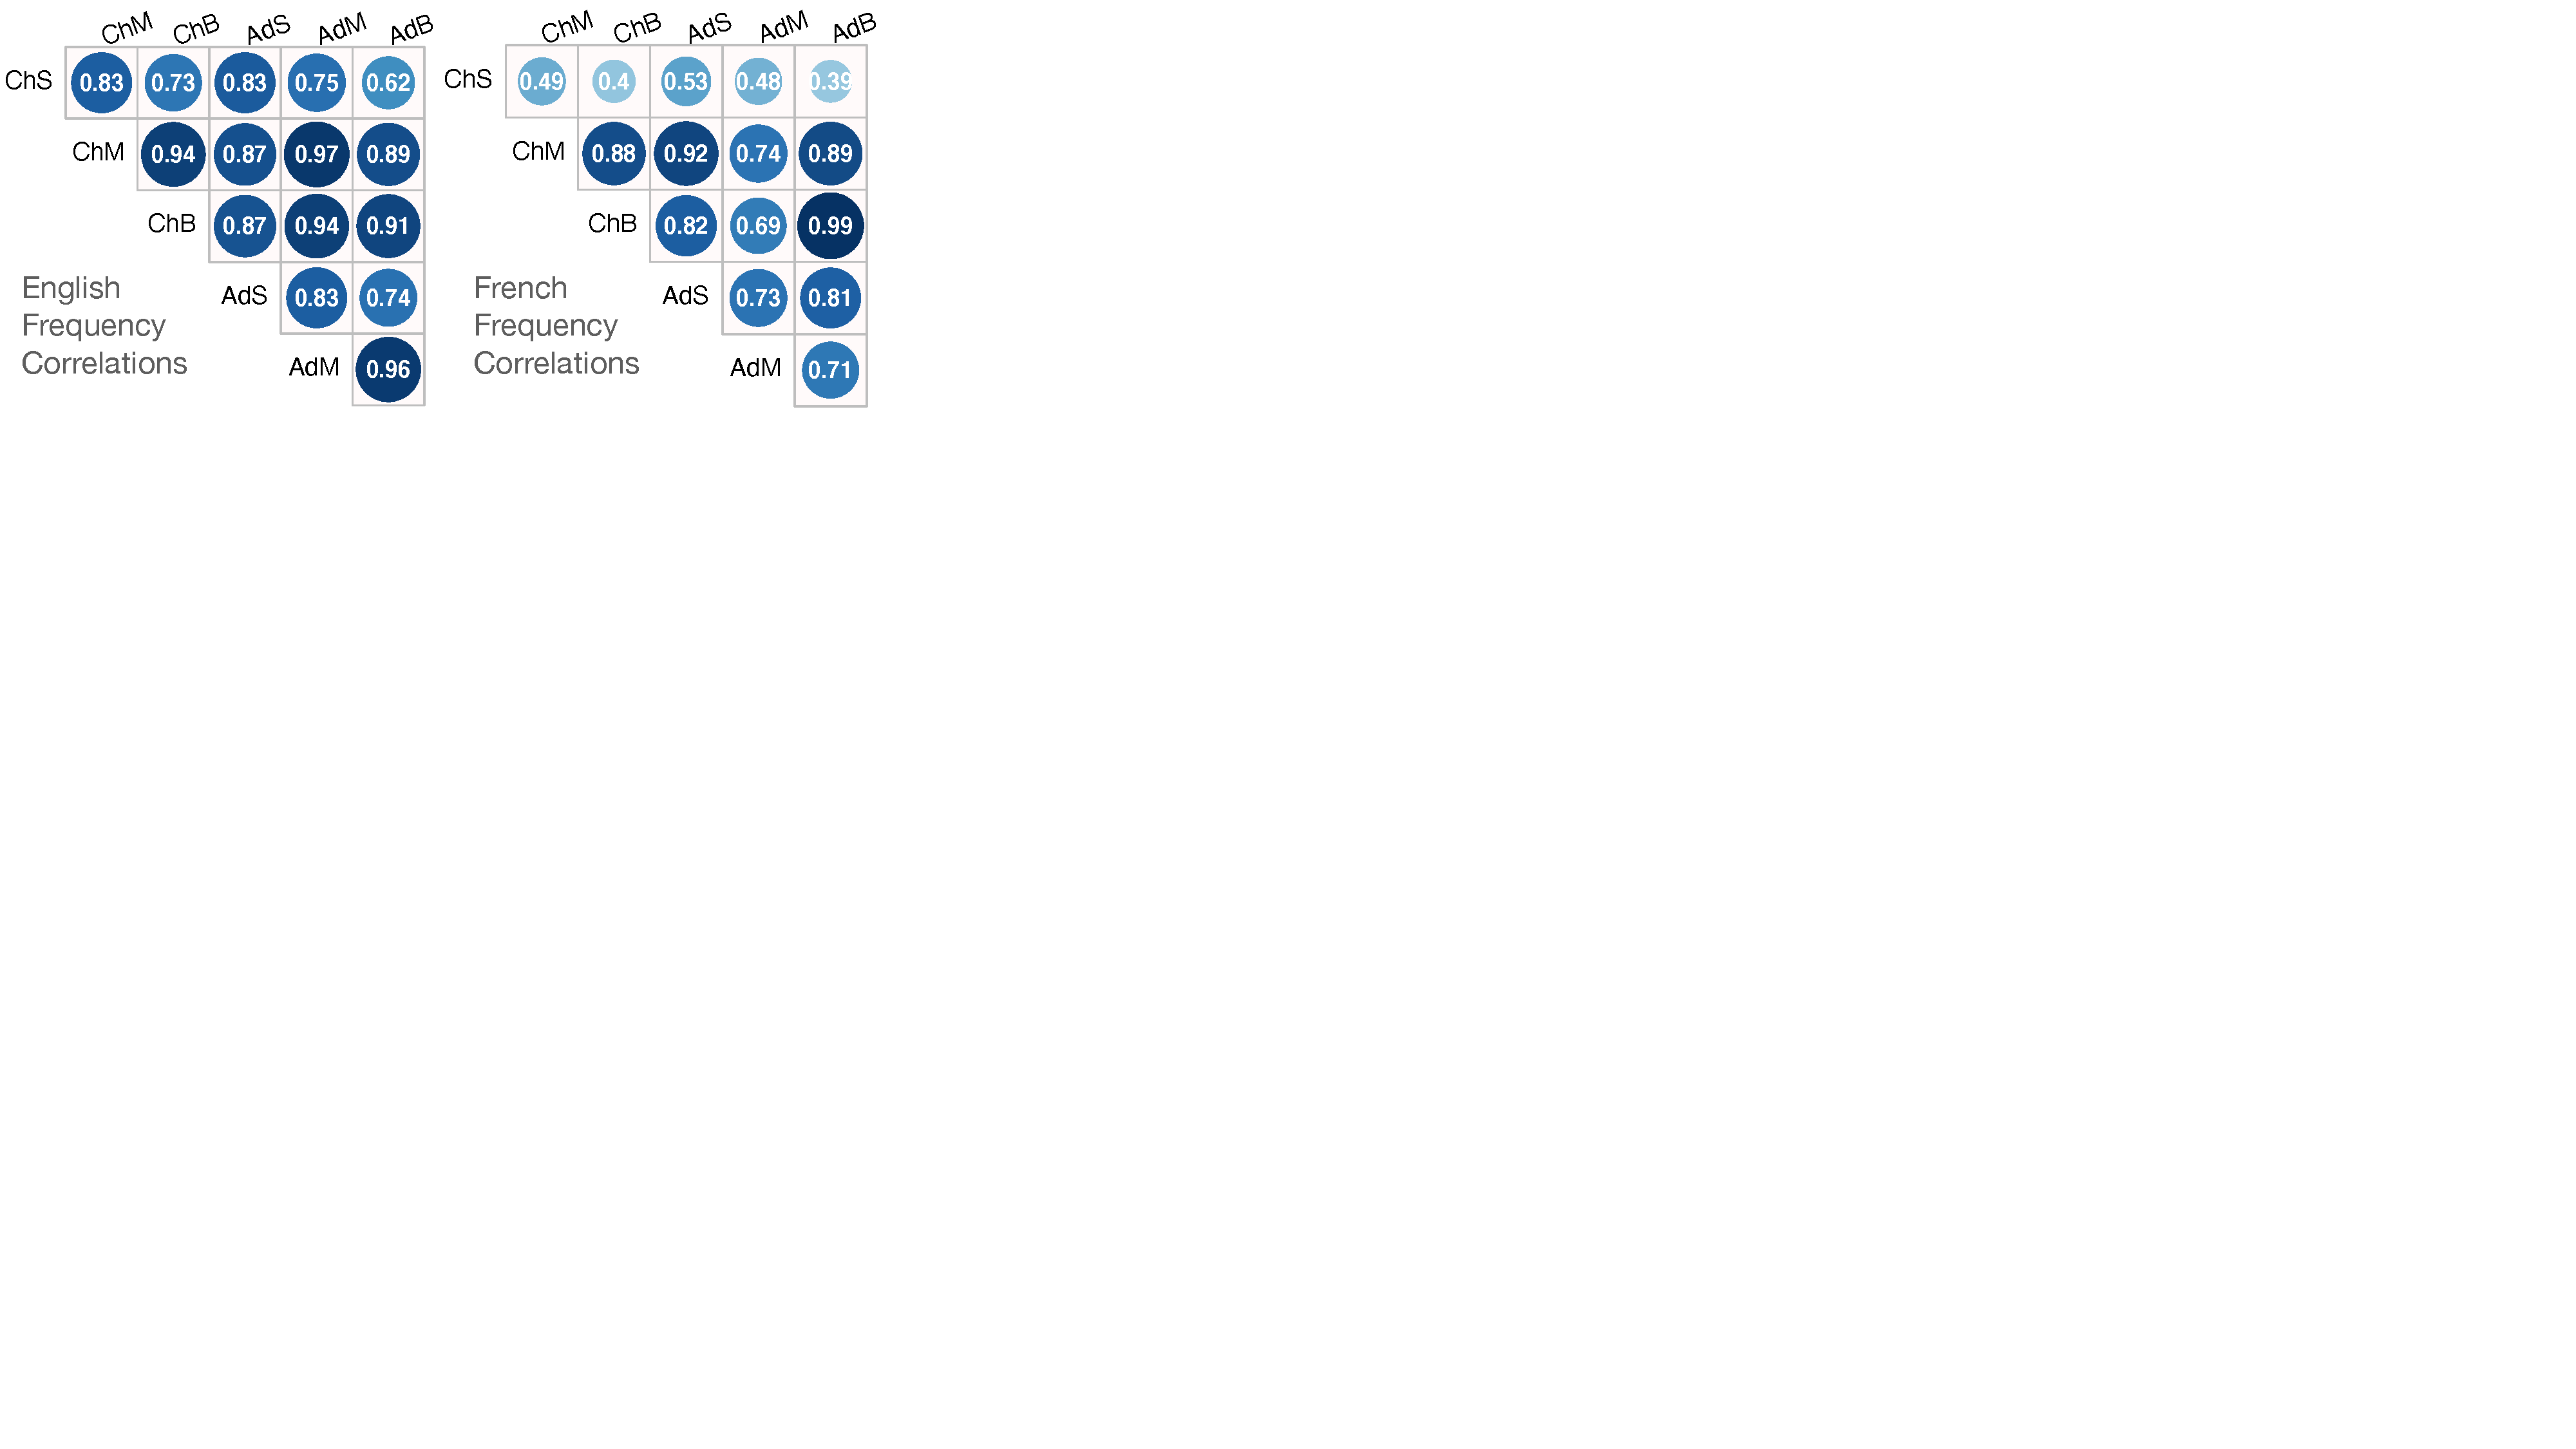
\includegraphics[width=\linewidth]{figs/corpus_freq_cors_hor} 

}

\caption[Word frequency correlations between different corpus sources for the matched CDI words in English (left) and French (right)]{Word frequency correlations between different corpus sources for the matched CDI words in English (left) and French (right).}\label{fig:fig1}
\end{figure}
\end{CodeChunk}

There are both register and source effects in both English and French.
Unsurprisingly, there were strong correlations across these different
corpora. We thus turned to PCA to disentangle these correlated
distributions and to understand their interrelations.

Table 1 shows the standard deviation (Std Dev) and proportion of
variance explained, both individually (Prop Var) and cumulatively (Cum
Prop Var) by the principal components (PC1-PC6) for each language. PC1
already explains the bulk of the variance (89\% for English and 68.8\%
for French), and PC2-PC4 each only capture an additional 2-4\% of the
variance for English, and 5-8\% for French. In total, the first four
components captured \textgreater98\% of the variance for English, and
\textgreater92\% for French.

Table 2 summarizes the eigenvectors of the principal components
(PC1-PC6) in relation to the original six frequency distributions for
English and French. The first PC is similar for both English and French,
and captures shared variance between all frequency sources, representing
words that are high or low frequency across registers and sources. This
component captures for example that `the' (EN), `le' (FR `the'), `et'
(FR `and') are frequent in spoken and written sources, whether directed
to adults or children. For English, PC2 (3.8\% of variance) mostly
captures child-directed speech, differentiating it from the other
registers. For example, words such as `peekaboo' are more present in
child-directed speech. For French, PC2 (9.8\% of variance) also captures
child-directed speech (e.g., `gâteau' = `sweet'), distinguishing it from
adult- and child-directed books.

For English, PC3 (3.2\% of variance) captures adult-directed speech,
differentiating it from the other registers. It captures words such as
`mower', `downtown' or `vitamins', frequent in discussions between
adults. For French, PC3 (7.2\%) similarly captures adult-directed
speech, with words such as \ldots{} For English, PC4 (2.3\% of variance)
captures the similarity of child- and adult-directed media,
distinguishing them from child- and adult-directed books. This component
captures that some words are very frequent in media in general, but
infrequent in books (e.g.~`camera', `TV') and vice-versa (e.g.~`none',
`beads', `poor'). For French, PC4 (6.4\% of variance) captures the
similarity of child- and adult-directed media (e.g.~`étoile' = `star'),
distinguishing them from child- and adult-directed speech
(e.g.~`voiture' = `car').

For English, PC5 (1.1\% of variance) captures child-directed speech,
distinguishing it from child-directed books. This component captures
that some words are very frequent in child-directed speech, but
infrequent in child-directed books (e.g.~`mommy', `juice') and
vice-versa (e.g.~`firetruck', `snowsuit'). For French, PC5 (4.9\%\% of
variance) distinguishes child-directed media (e.g.~`ferme' = `farm')
from adult-media (e.g.~`café'). Lastly, for English, PC6 (\textless1\%
of variance) is similar to PC5 in French (4.9\% of variance), capturing
child-directed media (.73), and distinguishing it in particular from
adult-directed media. This component captures that some words are very
frequent in child-directed media, but infrequent in adult-directed media
(e.g.~`penguin', `snowman') and vice versa (e.g.'drawer', `medicine').\\
For French, PC6 (3\%) distinguishes child-directed books (e.g.~`ours' =
`bear') from adult-directed books (e.g.~`tuer' = `kill').

In summary, the PCs align surprisingly well with particular dimensions
of the English frequency distributions: PC1 with overall frequency, PC2
with child-directed speech, PC3 with adult-directed speech, PC4 with
media vs.~books, PC5 with child-directed books vs.~speech, and PC6 with
adult- vs.~child-directed media. For French, we observe a similar
pattern of findings for PC1-PC4, although the amount of variance
explained is not quite the same. In PC5 and PC6, some frequency
differences across different registers are more pronounced for French
than for English.

\begin{CodeChunk}



\begin{table}[h]

\begin{center}
\begin{threeparttable}

\caption{\label{tab:pca-table}Importance of components from PCA for English (above) and French (below).}

\begin{tabular}{lllllll}
\toprule
 & \multicolumn{1}{c}{PC1} & \multicolumn{1}{c}{PC2} & \multicolumn{1}{c}{PC3} & \multicolumn{1}{c}{PC4} & \multicolumn{1}{c}{PC5} & \multicolumn{1}{c}{PC6}\\
\midrule
EN StdDev & 5.10 & 1.05 & 0.97 & 0.82 & 0.57 & 0.44\\
EN PropVar & 0.89 & 0.04 & 0.03 & 0.02 & 0.01 & 0.01\\
EN CumPropVar & 0.89 & 0.93 & 0.96 & 0.98 & 0.99 & 1.00\\
FR StdDev & 5.07 & 1.92 & 1.64 & 1.54 & 1.35 & 1.05\\
FR PropVar & 0.69 & 0.10 & 0.07 & 0.06 & 0.05 & 0.03\\
FR CumPropVar & 0.69 & 0.79 & 0.86 & 0.92 & 0.97 & 1.00\\
\bottomrule
\end{tabular}

\end{threeparttable}
\end{center}

\end{table}


\end{CodeChunk}

\begin{CodeChunk}



\begin{table}[tbp]

\begin{center}
\begin{threeparttable}

\caption{\label{tab:unnamed-chunk-2}Highlights from principal components' rotation in the original coordinate system.}

\begin{tabular}{lll}
\toprule
Order & \multicolumn{1}{c}{EN} & \multicolumn{1}{c}{FR}\\
\midrule
PC1 & Freq:-.31...-.52 & Freq:-.39...-.44\\
PC2 & ChS:.65; AdB:-.47 & ChS:.63; AdB:-.67\\
PC3 & AdS:.79; ChM:-.35 & AdS:.67; ChM:-.68\\
PC4 & M Ch:.40 A:.48; B\ \ Ch:-.63 A:-.44 & ChM:.55; ChS:-.63\\
PC5 & ChS:-.60; ChB:.53 & AdM:-.83; AdS:.50\\
PC6 & ChM:.73; AdM:-.53 & ChB:.79; AdB:.-56\\
\bottomrule
\end{tabular}

\end{threeparttable}
\end{center}

\end{table}


\end{CodeChunk}

\hypertarget{pca-based-age-of-acquisition-regression-q2}{%
\subsection{PCA-based Age of Acquisition Regression
(Q2)}\label{pca-based-age-of-acquisition-regression-q2}}

Next, we turned to question 2 asking how well these components predict
English- and French-learning children's early word learning. We
attempted a simple regression predicting each CDI word's mean AoA.
However, multicollinearity makes it unwise to include these raw
distributions in a regression, as the results would likely be unstable.
We verified that this was the case by running a regression predicting
AoA with log(word frequency) from each of the six distributions as
predictors.

The Variance Inflation Factor (VIF) estimates the inflation of the
variance of a regression coefficient when there is correlation between
predictors (Dodge, 2008). The higher the VIF for a predictor, the less
reliable the regression results are when that predictor is included. The
VIF for every distribution was \(>>1\) (and many \(>5\)), indicating
that these variables show strong multicollinearity which may compromise
the reliability of the regression results. We thus used the CDI items'
PCA loadings in lieu of the frequency distributions to predict AoA.
Figures showing the loadings of CDI items on PC1-PC4 by lexical class
vs.~the average age of acquisition (AoA; in months) can be found on
\href{https://osf.io/46gj2/?view_only=2db5950a96a44f289b6e778e60391662}{OSF}.

\begin{CodeChunk}



\begin{table}[h]

\begin{center}
\begin{threeparttable}

\caption{\label{tab:unnamed-chunk-4}Correlation of English AoA with PC loadings by lexical class.}

\begin{tabular}{lllllll}
\toprule
lexical\_class & \multicolumn{1}{c}{PC1} & \multicolumn{1}{c}{PC2} & \multicolumn{1}{c}{PC3} & \multicolumn{1}{c}{PC4} & \multicolumn{1}{c}{PC5} & \multicolumn{1}{c}{PC6}\\
\midrule
adjectives & -0.01 & -0.40 & -0.06 & -0.35 & 0.17 & 0.11\\
function\_words & 0.18 & -0.39 & 0.15 & -0.35 & 0.09 & -0.01\\
nouns & 0.40 & -0.27 & 0.20 & -0.24 & 0.33 & 0.02\\
other & -0.33 & -0.72 & 0.52 & -0.22 & 0.26 & -0.15\\
verbs & 0.17 & -0.31 & 0.30 & -0.11 & 0.20 & 0.04\\
\bottomrule
\end{tabular}

\end{threeparttable}
\end{center}

\end{table}


\end{CodeChunk}

\begin{CodeChunk}



\begin{table}[h]

\begin{center}
\begin{threeparttable}

\caption{\label{tab:unnamed-chunk-5}Correlation of French AoA with PC loadings by lexical class.}

\begin{tabular}{lllllll}
\toprule
lexical\_class & \multicolumn{1}{c}{PC1} & \multicolumn{1}{c}{PC2} & \multicolumn{1}{c}{PC3} & \multicolumn{1}{c}{PC4} & \multicolumn{1}{c}{PC5} & \multicolumn{1}{c}{PC6}\\
\midrule
adjectives & 0.00 & -0.11 & 0.06 & 0.00 & -0.06 & -0.05\\
function\_words & -0.04 & -0.02 & 0.05 & 0.06 & 0.00 & 0.03\\
nouns & 0.08 & -0.16 & -0.06 & -0.01 & -0.05 & 0.00\\
other & -0.11 & -0.32 & 0.05 & -0.02 & -0.03 & -0.10\\
verbs & 0.16 & -0.32 & -0.14 & 0.22 & -0.09 & 0.20\\
\bottomrule
\end{tabular}

\end{threeparttable}
\end{center}

\end{table}


\end{CodeChunk}

Given that past research has found that lexical class strongly modulates
influences of word frequency, we next examined the interaction of
lexical class (LC) with PC1 - PC6 in our regression. We also included
the number of letters as a predictor (Nletters) to help control for the
overall difficulty of each word. To determine if the inclusion of all
PCs was justified, we ran a series of ANOVAs building up from PC1 to
PC6--in decreasing order of the variance they accounted for in the
PCA\footnote{The R syntax for the sequence of regressions was
  \texttt{AoA}\(\sim\)\texttt{PC1*LC},
  \texttt{AoA}\(\sim\)\texttt{(PC1+PC2)*LC}, \ldots,
  \texttt{AoA}\(\sim\)\texttt{(PC1+PC2+PC3+PC4+PC5+PC6)*LC}, with noun
  as the baseline LC.}. The more complex model was always significantly
preferred, including up to the inclusion of PC6 (English:
\(R^2 = .584\), French: \(R^2 = .16\)). Figure 2 shows the coefficient
estimates with p\textless0.05 for both languages.

In general, we observe that registers and sources both matter for early
word learning. For English, PC1, PC2, PC3, PC4 and PC5 predict the age
of acquisition. Overall frequency (PC1) is a predictor; words which are
frequent in general are learned earlier than less frequent words.
Child-directed speech (PC2) is a negative predictor; words which are
frequent in this register are learned earlier on. On the contrary,
adult-directed speech (PC3) is a positive predictor; words which are
frequent in this register are learned later on. The frequency of words
in media distinguished from books is a predictor (PC4). Frequency of
words in child-directed speech distinguished from words in
child-directed books is also a significant predictor, with earlier
acquisition predicted for more speechy/less booky words. We also observe
that overall frequency interacts with lexical class, verbs, function
words and adjectives being learned later than nouns. PC2 interacts with
verbs, which are learned later than nouns. PC3 and PC6 each interacted
with function words, which are learned later than nouns.

For French, both registers and sources were important predictors of word
learning. PC1, PC2, PC3, PC4 and PC5 are significant predictors, showing
that speech, books, media and the child-directed register are all
important. Overall frequency (PC1) is a predictor; words which are
frequent in general are learned earlier than less frequent words. Book
frequency (PC2) is a predictor; words which are especially frequent in
books are learned later on. Child-directed speech (PC3) is a predictor;
words which are especially frequent in this register are learned earlier
on. PC4 includes words which are often found in media versus speech, and
PC5 includes words in child-directed versus adult-directed media.
Similarly to English, we also observe that overall frequency interacts
with lexical class, with verbs, function words, and adjectives being
learned later than nouns. Book frequency (PC2) interacts with verbs, and
child-directed media (PC5) interacted with function words. There is no
significant effect of word length.

In sum, in both languages, we observe that the predictive value of word
frequency comes from speech, media and book sources, and mostly the
child-directed register. The main differences across languages are that
for English, the difference and difficulty of adult-directed speech is
emphasized. For French, the difference and difficulty of text,
independent of register, is emphasized.

\begin{CodeChunk}
\begin{figure}[H]

{\centering 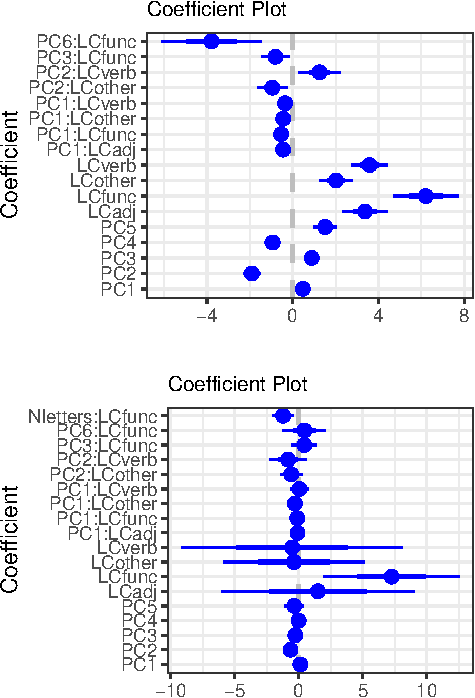
\includegraphics{figs/unnamed-chunk-6-1} 

}

\caption[Regression coefficients for predicting CDI AoAs with PCs and lexical class for English (top) and French (bottom)]{Regression coefficients for predicting CDI AoAs with PCs and lexical class for English (top) and French (bottom).}\label{fig:unnamed-chunk-6}
\end{figure}
\end{CodeChunk}

\hypertarget{combining-distributions-with-demographic-data-q3}{%
\subsection{Combining distributions with demographic data
(Q3)}\label{combining-distributions-with-demographic-data-q3}}

Previous findings relate SES status to book reading (Shen \& Del Tufo,
2022), which is in turn related to better language skills (Bus, Van
Ijzendoorn, \& Pellegrini, 1995). This suggests that the vocabulary
composition of children from higher-SES households may be better
predicted by the word frequencies seen in child-directed books, rather
than those from child-directed speech. To test this idea, we did an
exploratory logistic regression using the first four PCs to predict the
number of children in Wordbank who produce or don't produce each item,
along with interactions of mother's education and children's age. Due to
lack of maternal education data for French data, we focus on American
English-learning children. American English data from Wordbank contained
2,776 CDI:WS administrations with mother's education coded as a factor
(baseline (0): no more than secondary education (N=547), 1 for some/all
college (N=1483), and 2 for at least some graduate school (N=746)).

There were significant main effects of age, mother's education, and
PC1-PC4 (all \(p<.001\)). There were significant interactions of age
with mother's education (\(p<.001\)), PC2 (\(p<.001\)), and PC4
(\(p=.009\)). There were significant interactions of mother's education
with PC1-PC3 (all \(p<.001\)), shown in Figure 3.

\begin{table}[ht]
\centering
\begin{tabular}{rrrrr}
  \hline
 & Beta & SE & t-val & p-val \\ 
  \hline
(Intercept) & -5.33 & 0.05 & -117.54 & 0.00 \\ 
  age & 0.21 & 0.00 & 204.85 & 0.00 \\ 
  MotherEdCollege & -1.54 & 0.03 & -53.74 & 0.00 \\ 
  MotherEdGraduate & -1.76 & 0.03 & -55.35 & 0.00 \\ 
  PC1 & 0.07 & 0.01 & 7.39 & 0.00 \\ 
  PC2 & 0.31 & 0.04 & 7.53 & 0.00 \\ 
  PC3 & -0.29 & 0.05 & -6.08 & 0.00 \\ 
  PC4 & 0.15 & 0.05 & 2.81 & 0.00 \\ 
  age:MotherEdCollege & 0.07 & 0.00 & 59.18 & 0.00 \\ 
  age:MotherEdGraduate & 0.09 & 0.00 & 67.84 & 0.00 \\ 
  age:PC1 & -0.00 & 0.00 & -7.94 & 0.00 \\ 
  age:PC2 & -0.01 & 0.00 & -6.89 & 0.00 \\ 
  age:PC3 & 0.00 & 0.00 & 3.92 & 0.00 \\ 
  age:PC4 & 0.00 & 0.00 & 3.03 & 0.00 \\ 
   \hline
\end{tabular}
\caption{Regression coefficients for predicting English CDI items using PCs and mother's education.} 
\end{table}

\begin{CodeChunk}
\begin{figure}[H]

{\centering 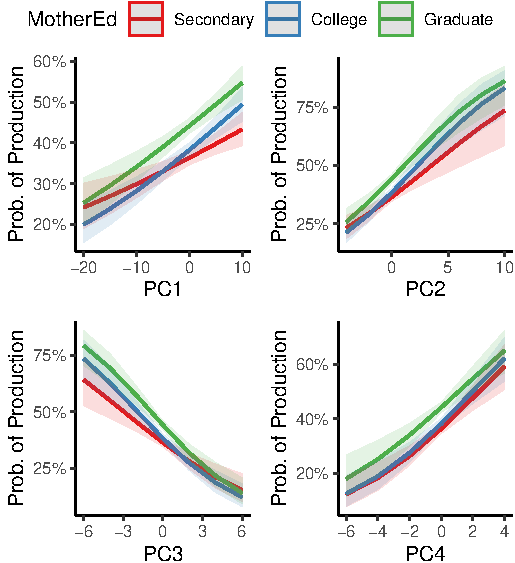
\includegraphics{figs/unnamed-chunk-7-1} 

}

\caption[Predicted effects of maternal education and PC1-PC4 on the probability of children producing CDI words]{Predicted effects of maternal education and PC1-PC4 on the probability of children producing CDI words.}\label{fig:unnamed-chunk-7}
\end{figure}
\end{CodeChunk}

\hypertarget{discussion}{%
\section{Discussion}\label{discussion}}

We set out to investigate the sources of linguistic input and registers
that children may experience, using word frequency distributions
garnered from child-directed and adult-directed corpora of speech,
books, and media (TV and movies). We found the principal components
(PCs) of these distributions, and described how these PCs capture
variation both in adult- vs.~child-directedness, as well as between
modalities (e.g., books and speech).

Our findings show that PC1 explains 95\% of the variance in frequency
distributions. This means that most frequency is shared by the different
sources, thus accounted for by that one component. Moreover, multiple
components are predictive of children's age of acquisition of words from
the CDI. Speech, but also books and media are all relevant in predicting
age of acquisition, as well as child-directed speech. This suggests that
children's environmental exposure to different language sources, even
when these include books or even media, could impact their word learning
trajectory. It is somewhat surprising that even sources of input that
young children rarely encounter (e.g., adult-directed books) contribute
significantly to predicting variation in children's early word learning.

We also used English Wordbank data to examine how well the frequency
components combine with mother's education--a measure of SES that has
been found in the past to be positively related to early word learning,
and to more child-directed reading--to predict children's early word
learning. This analysis revealed significant contributions of multiple
PCs, as well as the interaction of mother's education with PC1 (overall
frequency), PC2 (child-directed speech), and PC3 (adult-directed
speech), but not of the child-directed books component (PC4).

These findings are important for educational reasons and could inform
future interventions on the importance of including language from
different sources. A target for future research is to predict individual
children's learning of particular words using these principal
components, in combination with parent-reported measures of how much
time their child spends daily receiving input from each of the input
sources ({[}adult- vs.~child-directed{]} x {[}books, media, and
speech{]}).

Finally, there was overwhelming similarity of word frequency
distributions from different sources and their predictive value in
English and French data, which supports the robustness of the results.
At the same time, these distributions show systematic variation--at
least in English and in French, which can predict some of the variation
in children's early word learning. We should also notice that different
data and corpus sizes were used to represent the sources for each
language. Differences could also be partly attributed to this e.g., the
French corpora were composed of several smaller ones, due to the lack of
large accessible corpora, and had slightly different use e.g.~small
stories in French, large books in English.

By better understanding the similarity and differences between word
frequencies children experience in different contexts, future research
in this vein holds the promise to predict individual differences in
children's early word learning on the basis of their daily routines.

\hypertarget{acknowledgements}{%
\section{Acknowledgements}\label{acknowledgements}}

{[}Redacted for anonymous review.{]}

\hypertarget{references}{%
\section{References}\label{references}}

\setlength{\parindent}{-0.1in} 
\setlength{\leftskip}{0.125in}

\noindent

\hypertarget{refs}{}
\begin{CSLReferences}{1}{0}
\leavevmode\vadjust pre{\hypertarget{ref-ambridge2015ubiquity}{}}%
Ambridge, B., Kidd, E., Rowland, C. F., \& Theakston, A. L. (2015). The
ubiquity of frequency effects in first language acquisition.
\emph{Journal of Child Language}, \emph{42}(2), 239--273.

\leavevmode\vadjust pre{\hypertarget{ref-andre2010mise}{}}%
André, V., \& Canut, E. (2010). Mise {à} disposition de corpus oraux
interactifs: Le projet TCOF (traitement de corpus oraux en fran{ç}ais).
\emph{Pratiques. Linguistique, Litt{é}rature, Didactique}, (147-148),
35--51.

\leavevmode\vadjust pre{\hypertarget{ref-balthasar2005plateforme}{}}%
Balthasar, L., \& Bert, M. (2005). La plateforme corpus de langues
parl{é}es en interaction(CLAPI). Historique, {é}tat des lieux,
perspectives. \emph{Lidil. Revue de Linguistique Et de Didactique Des
Langues}, (31), 13--33.

\leavevmode\vadjust pre{\hypertarget{ref-braginsky2019consistency}{}}%
Braginsky, M., Yurovsky, D., Marchman, V. A., \& Frank, M. C. (2019).
Consistency and variability in children's word learning across
languages. \emph{Open Mind}, \emph{3}, 52--67.

\leavevmode\vadjust pre{\hypertarget{ref-branca2012discours}{}}%
Branca-Rosoff, S., Fleury, S., Lefeuvre, F., \& Pires, M. (2012).
Discours sur la ville. Pr{é}sentation du corpus de fran{ç}ais parl{é}
parisien des ann{é}es 2000 (CFPP2000). \emph{Article En Ligne,
Http://Cfpp2000. Univparis3. Fr/Articles. Html}.

\leavevmode\vadjust pre{\hypertarget{ref-bus1995joint}{}}%
Bus, A. G., Van Ijzendoorn, M. H., \& Pellegrini, A. D. (1995). Joint
book reading makes for success in learning to read: A meta-analysis on
intergenerational transmission of literacy. \emph{Review of Educational
Research}, \emph{65}(1), 1--21.

\leavevmode\vadjust pre{\hypertarget{ref-charlesworth2021gender}{}}%
Charlesworth, T. E., Yang, V., Mann, T. C., Kurdi, B., \& Banaji, M. R.
(2021). Gender stereotypes in natural language: Word embeddings show
robust consistency across child and adult language corpora of more than
65 million words. \emph{Psychological Science}, \emph{32}(2), 218--240.

\leavevmode\vadjust pre{\hypertarget{ref-dawson2021features}{}}%
Dawson, N., Hsiao, Y., Wei Ming Tan, A., Banerji, N., \& Nation, K.
(2021). Features of lexical richness in children's books: Comparisons
with child-directed speech. \emph{Language Development Research}.

\leavevmode\vadjust pre{\hypertarget{ref-dodge2008concise}{}}%
Dodge, Y. (2008). \emph{The concise encyclopedia of statistics}.
Springer Science \& Business Media.

\leavevmode\vadjust pre{\hypertarget{ref-fenson1994variability}{}}%
Fenson, Larry, Dale, P. S., Reznick, J. S., Bates, E., Thal, D. J.,
Pethick, S. J., \ldots{} Stiles, J. (1994). Variability in early
communicative development. \emph{Monographs of the Society for Research
in Child Development}, i--185.

\leavevmode\vadjust pre{\hypertarget{ref-fenson2007}{}}%
Fenson, L., Marchman, V. A., Thal, D. J., Dale, P. S., Reznick, J. S.,
\& Bates, E. (2007). \emph{{M}ac{A}rthur-{B}ates {C}ommunicative
{D}evelopment {I}nventories: User's guide and technical manual (2nd
ed.)}. Baltimore, MD: Brookes.

\leavevmode\vadjust pre{\hypertarget{ref-fernald2013ses}{}}%
Fernald, A., Marchman, V. A., \& Weisleder, A. (2013). SES differences
in language processing skill and vocabulary are evident at 18 months.
\emph{Developmental Science}, \emph{16}(2), 234--248.

\leavevmode\vadjust pre{\hypertarget{ref-frank2017wordbank}{}}%
Frank, M. C., Braginsky, M., Yurovsky, D., \& Marchman, V. A. (2017).
Wordbank: An open repository for developmental vocabulary data.
\emph{Journal of Child Language}, \emph{44}(3), 677--694.

\leavevmode\vadjust pre{\hypertarget{ref-goodman2008}{}}%
Goodman, J. C., Dale, P. S., \& Li, P. (2008). Does frequency count?
Parental input and the acquisition of vocabulary. \emph{Journal of Child
Language}, \emph{35}(3), 515--531.

\leavevmode\vadjust pre{\hypertarget{ref-hart1995meaningful}{}}%
Hart, B., \& Risley, T. R. (1995). \emph{Meaningful differences in the
everyday experience of young american children.} Paul H Brookes
Publishing.

\leavevmode\vadjust pre{\hypertarget{ref-hill2015goldilocks}{}}%
Hill, F., Bordes, A., Chopra, S., \& Weston, J. (2015). The goldilocks
principle: Reading children's books with explicit memory
representations. \emph{arXiv Preprint arXiv:1511.02301}.

\leavevmode\vadjust pre{\hypertarget{ref-hoff2003specificity}{}}%
Hoff, E. (2003). The specificity of environmental influence:
Socioeconomic status affects early vocabulary development via maternal
speech. \emph{Child Development}, \emph{74}(5), 1368--1378.

\leavevmode\vadjust pre{\hypertarget{ref-macwhinney2000childes}{}}%
MacWhinney, B. (2000). \emph{The CHILDES project: Tools for analyzing
talk. Transcription format and programs} (Vol. 1). Psychology Press.

\leavevmode\vadjust pre{\hypertarget{ref-montag2015words}{}}%
Montag, J. L., Jones, M. N., \& Smith, L. B. (2015). The words children
hear: Picture books and the statistics for language learning.
\emph{Psychological Science}, \emph{26}(9), 1489--1496.

\leavevmode\vadjust pre{\hypertarget{ref-rowe2012longitudinal}{}}%
Rowe, M. L. (2012). A longitudinal investigation of the role of quantity
and quality of child-directed speech in vocabulary development.
\emph{Child Development}, \emph{83}(5), 1762--1774.

\leavevmode\vadjust pre{\hypertarget{ref-shen2022parent}{}}%
Shen, Y., \& Del Tufo, S. N. (2022). Parent-child shared book reading
mediates the impact of socioeconomic status on heritage language
learners' emergent literacy. \emph{Early Childhood Research Quarterly},
\emph{59}, 254--264.

\end{CSLReferences}

\bibliographystyle{apacite}


\end{document}
